\documentclass[two column, twoside, a4paper]{article}

\usepackage[utf8]{inputenc}
\usepackage{dblfloatfix}
\usepackage{subcaption}
\usepackage{float}
\usepackage[backend=biber, maxbibnames=3, style=nature, autocite=inline]{biblatex}
\usepackage[polish]{babel}
\usepackage[T1]{fontenc}
\usepackage{fancyhdr}
\usepackage{titlesec}
\usepackage{blindtext}
\usepackage{cuted}
\usepackage{tikz}
\usepackage[most]{tcolorbox}
\usepackage[columnsep = 1cm,
	        lmargin = 0.6in,
	        rmargin = 0.4in,
	        tmargin = 0.5in,
	        bmargin = 0.65in,
	        headsep = \baselineskip]{geometry}

\addbibresource{$BIB}

% Custom commands
\newcommand*\circled[1]{\tikz[baseline=(char.base)]{
            \node[shape=circle,draw,inner sep=2pt, color = orange!90!white] (char) {#1};}}

\newcommand{\maldi}{MALDI-TOF MS }

% Section Formatting
\titleformat{\section}
{\sc \bfseries \Large}
{}
{0em}
{}[\titlerule]

\titleformat{\subsection}
{\bfseries \large}
{}
{0em}
{}

\titleformat{\subsubsection}
{\bfseries}
{}
{0em}
{}

% Box formatting
\tcbset{enhanced, colback=orange!15!white, boxrule = 1pt, coltitle = orange!90!white, colbacktitle = orange!15!white, colframe= orange!50!white}

\pagestyle{fancy}
\fancyhf{}
\fancyhead[RE, LO]{Szkoła Główna Gospodarstwa Wiejskiego}
\fancyhead[LE, RO]{Biotechnologia}
\fancyfoot[RE, LO]{Jakub J. Guzek}
\fancyfoot[LE, RO]{\thepage}
\fancyfoot[CE,CO]{Zastosowanie spektrometrii mas w diagnostyce mikrobiologicznej}
\renewcommand{\footrulewidth}{0.05pt}

\begin{document}

\begin{strip}
	{\sc \bfseries \LARGE \fontfamily{phv}\selectfont Zastosowanie spektrometrii mas w diagnostyce

	\vspace{2pt} mikrobiologicznej} \vspace{\baselineskip}

{\bfseries \large Jakub J. Guzek}

{Szkoła Główna Gospodarstwa Wiejskiego, Biotechnologia, Nr. albumu: 195528}\vspace{\baselineskip}

\hrule
\end{strip}

\textbf{Spektroskopia mas jest jedną z opracowanych w XXw. metod analizy cząsteczek, umożliwiającą poznanie masy cząsteczki i częściowo wnioskowania o jej strukturze na podstawie widma mas. Początkowo była to metoda stosowana wyłącznie do badania prostych cząsteczek organicznych z czasem jednak była adoptowana do coraz bardziej złożonych związków, a pod koniec XXw. pojawiły się propozycje użycia jej na całych organizmach (konkretnie na komórkach bakteryjnych). Opracowane do badania tą metodą sposoby jonizacji próbki i analizy wyników takie jak MALDI-TOF MS, czy ESI MS, umożliwiają identyfikację i klasyfikację mikroorganizmów na podstawie uzyskanego widma -- które stanowi niejako ,,odcisk palca'' danego mikroorganizmu -- nawet do poziomu gatunku, czy w niektórych przypadkach do poziomu serogrupy\autocite{Biswas2013}.}


\begin{figure}[t]
\begin{tcolorbox}
	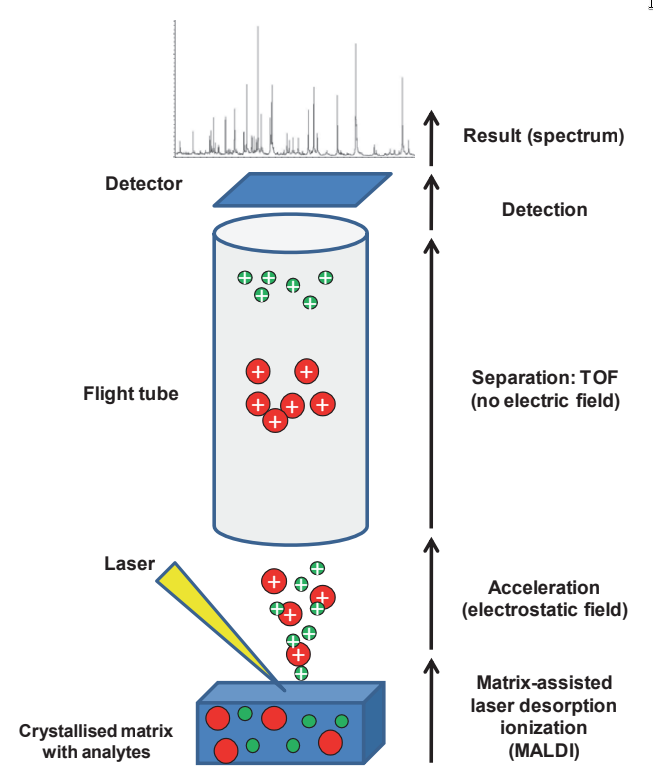
\includegraphics[width=\textwidth]{./figures/maldi-tof.png}
	\caption{Próbka mieszana jest z organiczną macierzą na przewodzącej, metalowej płytce. Po krystalizacji materiału mikrobiologicznego z macierzą płytka poddawana jest działaniu pulsów lasera. Zdesorbowane i zjonizowane cząsteczki są przyspieszane w polu elektrostatycznym i wystrzelane przez tubę w stronę detektora. Lecą w próżni. Lżejsze jony poruszają się szybciej niż cięższe, więc zostają podzielone według czasu ich przelotu. Dzięki temu powstaje spektrum złożone z pików stosunków mas do ładunków, o różnych intensywnościach. To spektrum jest swoistym ,,odciskiem palca'' danego mikroorganizmu i porównywane jest do bazy danych w celu identyfikacji drobnoustroju. (Na postawie: Croxatto, 2012)}\label{fig::maldi-tof.png}
\end{tcolorbox}
\vspace{-1.8em}
\end{figure}

\section{Wstęp}

Jedną z pierwszych szeroko stosowanych w diagnostyce mikrobiologicznej metod spektrometrii mas jest \textbf{jonizacja laserem wspomagana matrycą -- analiza czasu przelotu} (\textit{matrix-assisted laser desorption ionization time-of-flight mass spectrometry}, MALDI-TOF MS). Generuje ona widma mas charakterystyczne dla danego mikroorganizmu, umożliwiające identyfikację na poziomie rodzaju, gatunku lub nawet szczepu czy serogrupy\autocite{Biswas2013, Brown2019, Croxatto2012}.

Pierwszym etapem w tej metodzie jest jonizacja próbki. Próbka, którą są albo wyizolowane peptydy, albo całe mikroorganizmy, jest adsorbowana na organicznej matrycy. Matrycą taką zwykle jest kwas synapinowy, kwas ferulowy lub kwas 2,5-dihydroksybenzoesowy. Po adsorpcji jest poddawana działaniu impulsów z lasera UV. Wzbudzenie jonizuje cząsteczki matrycy i prowadzi do powstawania jonów molekularnych i desorpcji składników próbki. Składniki te są transferowane do zjonizowanej fazy gazowej, a następnie przyspieszane w polu elektrycznym urządzenia spektrometru. Czas potrzebny na przelot zjonizowanych cząstek jest proporcjonalny do pierwiastka ze stosunku ich masy i ładunku $m/z$. Na podstawie czasu przelotu określane jest właśnie $m/z$. Ponieważ ładunek jonu wynosi w całkowitej większości przypadków jeden (dodatnie lub ujemne) to znając czas jego przelotu, można łatwo obliczyć jego masę. Rejestracja przelotu jonów z próbki jaką jest cały mikroorganizm daje widmo masy charakterystyczne dla danej próbki i mające unikalne piki, umożliwiające identyfikację i klasyfikację\autocite{Brown2019, Croxatto2012}.


Istnieją też inne sposoby prowadzenia tego typu spektrometrii takie jak np. \textbf{technika jonizacji przez rozpylenie w polu elektrycznym} (\textit{electrospray-ionization}, ESI) lub \textbf{technika jonizacji chemicznej} (\textit{chemical ionization} CI)\autocite{Brown2019, Croxatto2012}

Prócz tego istnieją również inne rodzaje analizatorów mas takie jak \textbf{kwadrupol}, \textbf{hybrydowy kwadrupol w analizą czasu przelotu} (\textit{hybrid quadrupole TOF}, Q-Q-TOF), lub \textbf{analizator cyklotronowego rezonansu jonów z fourierowską transformacją wyników} (\textit{Fourier-transform ion cyclotron resonanse}, FT-ICR)\autocite{Brown2019}.

\begin{figure*}[t]
\begin{tcolorbox}
	\begin{subfigure}{0.491\textwidth}
		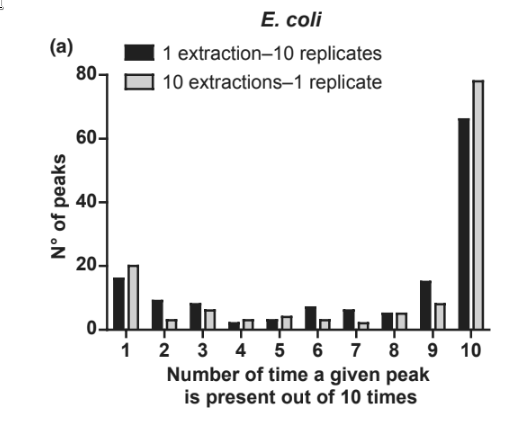
\includegraphics[width=\textwidth]{./figures/reprod1.png}
	\end{subfigure}
	\begin{subfigure}{0.5\textwidth}
		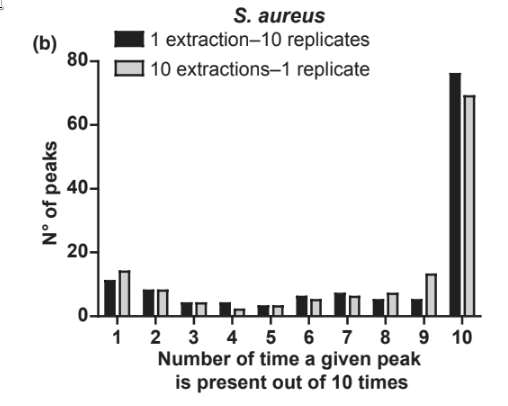
\includegraphics[width=\textwidth]{./figures/reprod2.png}
	\end{subfigure}
	\caption{Wewnątrzlaboratoryjna powtarzalność wyników sprawdzona poprzez mierzenie ilości pików w dwóch eksperymentach. W pierwszym ekstrakcja przy użyciu etanolu/kwasu mrówkowego zostawała zastosowana dla \textit{E. coli} (a) i \textit{S. aureus} (b). 10 namnożonych próbek z jednej ekstrakcji zostało zbadanych przy użyciu \maldi. W drugim przeprowadzone zostało 10 niezależnych ekstrakcji i jedna próbka każdej z nich została zbadana przy użyciu \maldi. Z obydwu eksperymentów wybrane zostało 100 najsilniejszych pików i zliczone zostało ile razy dany pik pojawił się w 10 próbach przeprowadzonych w obydwu eksperymentach. (Na podstawie Croxatto, 2012)}\label{fig:reprod}
\end{tcolorbox}
\end{figure*}

\section{Biomarkery i analiza daych}

Wyniki uzyskane przy użyciu techniki MALDI-TOF i niektórych jej pokrewnych są to charakterystyczne widma mas, unikalne dla danej próbki. Daje się jednak w takich widmach zidentyfikować powtarzalne piki, pozwalające na identyfikację mikroorganizmów poddanych \maldi, poprzez porównanie otrzymanych widm z widmami obecnymi w bazach danych, które są często dostępne wraz ze spektrometrami.

Charakterystyczne są zwłaszcza piki korespondujące do zasadowych białek, o lekko hydrofobowym charakterze, których zawartość w komórce jest relatywnie wysoka. Białkami o takich cechach jest duża ilość białek rybosomalnych, białek asocjujących z DNA oraz białek szoku termicznego. Peptydy te stanowią więc biomarkery w tej metodzie i umożliwiają identyfikację mikroorganizmów.

Metoda \maldi ma dobre rezultaty dla dużej części testowanych drobnoustrojów i zwykle misidentyfikację można przypisać niewystarczającej liczbie spektrów dla danego mikroorganizmu obecnych w bazie danych, lub specyfice danego organizmu\autocite{Croxatto2012}

\section{Zastosowanie MALDI-TOF MS}

\maldi umożliwia wielokrotne skrócenie czasu potrzebnego do identyfikacji mikroorganizmów zawartych zarówno w hodowlach jak i np. w krwi pacjenta w stosunku do metod bacujących na fenotypie lub biochemii. Dodatkowo jest wielokrotnie tańsze i mniej pracochłonne niż wiele metod biochemicznych lub molekularnych.

Problematyczna jest konieczność ścisłego trzymania się protokołu przygotowywania próbki w celu uzyskania jak najdokładniejszej identyfikacji, gdyż jest to metoda niezwykle czuła na nawet najmniejsze zmiany w środowisku hodowlanym drobnoustrojów. Problem ten częściowo rozwiązuje zastosowanie algorytmów bazujących na uczeniu maszynowym, które przy zastosowaniu bazy danych o zadowalających zasobach są zdolne do identyfikacji nawet próbek poddanych działaniu różnych warunków środowiska\autocite{Croxatto2012}.

Bardzo istotna jest możliwość zastosowania techniki \maldi do identyfikacji i klasyfikacji\footnote{przy użyciu odpowiednich metod komputerowych i statystycznych} mikroorganizmów kłopotliwych w hodowli takich jak anaeroby z rodzajów \textit{Bacterioides}, \textit{Prevotella}, \textit{Porphyromonas}, \textit{Peptostreptococcus}, \textit{Anaerococcus}, \textit{Clostridium}, \textit{Actinomyces}, \textit{Propionibacterium} i \textit{Veillonella}; wolnorosnące auksotrofy z rodzajów \textit{Bartonella}, \textit{Legionella} i  \textit{Coxiella}; oraz mykobakterie. Możliwość przyspieszenia identyfikacji wymienionych organizmów ma szczególne znaczenie dla diagnotyki klinicznej, gdyż wiele z nich powoduje poważne choroby (patogenne kostridia, \textit{Legionella penumopila}, wywołująca gorączkę Q \textit{Coxiella burnetti}, czy \textit{Mycobacterium tuburcolosis} -- czynnik etiologiczny gruźlicy i \textit{Mycobacterium leprae} -- czynnik etiologiczny trądu), a jest trudne do zidentyfikowania z wielu względów. Niektóre z nich rosną niezwykle powoli. Inne są niezwykle trudne do identyfikacji przy użyciu metod biochemicznych lub obserwacji cech fenotypowych, a zastosowanie metod molekularnych jest pracochłonne, czasochłonne i nieraz wymaga uprzedniego określenia z jaką grupą organizmów się pracuje\autocite{Biswas2013}.

Wszystkie wyżej wymienione mikroorganizmy mogą być zidentyfikowane przy \maldi przy zastosowaniu odpowiednich protokołów dotyczących przygotowania próbek, lub analizy danych, przy czym może wymagać czasem zastosowania technik pomocniczych w celu potwierdzenia wyniku jak np. w wypadku \textit{Coxiella burnetti}\autocite{Biswas2013, Croxatto2012}

Metody spektrometrii umożliwiają także identyfikację grzybów strzępkowych, dermatofitów i drożdży, przy czym jest to nieco bardziej problematyczne w wypadku pierwszych dwóch gdyż mają one o wiele bardziej heterogenną strukturę niż większość bakterii, co skutkuje koniecznością modyfikacji procedur przy pracy z nimi\autocite{Croxatto2012}

\section{Podsumowanie}

Metody spektrometrii umożliwiają znaczące skrócenie czasu potrzebnego do identyfikacji mikroorganizmów (z wielu godzin do nawet kilku minut\footnote{nie licząc czasu potrzebnego do ewentualnej hodowli drobnoustrojów, gdyż jest to konieczne, również w metodach ,,tradycyjnych''}), a także zmniejszenie koniecznego do tego nakładu pracy. Pociąga za sobą także obniżenie kosztów takiej identyfikacji oraz daje lepsze prognozy dla identyfikacji organizmów neutralnych biochemicznie i trudnych do rozpoznania fenotypowo, co ma niebagatelne znaczenie w diagnostyce klinicznej i weterynaryjnej. Przyspieszenie procesu identyfikacji patogenu jest niezwykle znaczące dla kuracji pacjenta.

Spektrometria umożliwia także do pewnego stopnia badanie proteomu i tego jak jego struktura zmienia się w różnych warunkach.

\printbibliography

\end{document}
